\header{
    \headtitle{Chantons pour passer le temps} \label{chantons-pour-passer-le-temps}
    %
    
    \insertComment{Chanson traditionelle de Normandie avec adaptations en fonction des régions.}{Considérée ancienne dans "La clé de Caveau" (1811).}
}
\vspace{-0.3cm}
\enluminure{4}{\href{https://www.youtube.com/watch?v=x1008sA5KY4}{C}}{hantons} pour passer le temps
\\Les amours charmants d'une belle fille,
\\Chantons pour passer le temps,
\\D'une belle fille les amours charmants.
\\Aussitôt que son amant l'eût prise,
\\Aussitôt elle changea de mise,
\\Et prit l'habit de matelot,
\\Et vint s'embarquer à bord du navire,
\\Et prit l'habit de matelot,
\\Et vint s'embarquer à bord du vaisseau.
\\\\Le capitaine, enchanté
\\D'avoir à son bord un si beau jeune homme,
\\Le Capitaine, enchanté,
\\Lui dit: "A mon bord, je vais te garder.
\\Tes beaux yeux, ton joli visage,
\\Tes cheveux et ton joli corsage,
\\Me font toujours me rappeler
\\D'anciennes amours avec une belle;
\\Me font toujours me rappeler
\\Une beauté de jadis que j'ai tant aimée !"
\\\\"Monsieur vous vous moquez de moi,
\\Vous me badinez, vous me faites rire;
\\Je n'ai ni frère, ni parents,
\\Et ne suis pas née au port de Lorient.
\\Je suis née à la Martinique,
\\Je suis même z' une enfant unique
\\Et c'est un vaisseau hollandais
\\Qui m'a débarquée en venant des îles,
\\Et c'est un vaisseau hollandais,
\\Qui m'a débarquée au port de Calais !"
\breakpage 
Ils ont ainsi vécu sept ans,
\\Sur le bâtiment sans se reconnaître;
\\Ils ont ainsi vécu sept ans,
\\Se sont reconnus au débarquement.
\\"Puisqu'enfin l'amour nous rassemble,
\\Nous allons nous marier ensemble;
\\L'argent que nous avons gagné,
\\Il nous servira dans notre ménage;
\\L'argent que nous avons gagné,
\\Il nous servira pour nous marier !"
\\\\Celui-là qu'a fait la chanson.
\\C'est le gars Camus, le gabier de misaine,
\\Celui-là qu'a fait la chanson,
\\C'est le gars Camuse le gabier d'artimon.
\\Oh ! matelots larguez la grand-voile,
\\Aux palans, que tout le monde y soye;
\\Et vire et vire vire donc,
\\Sinon t'auras pas de vin plein ta bedaine,
\\Et vire et vire vire donc,
\\Ou t'auras pas ta ration dans le bedon.
\begin{center}
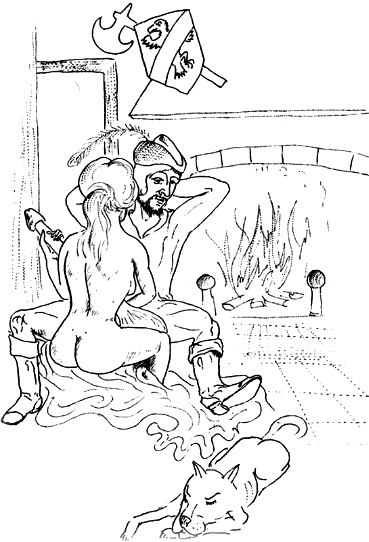
\includegraphics[width=0.5\textwidth]{images/chantons.jpg}
\end{center}

\breakpage